\section{Array performance}

The aim of this section is to evaluate the beamforming array performance. In \autoref{} it was discovered that the pressure in front of the beamforming array do not act linear form \SI{60}{\hertz} to \SI{300}{\hertz} and therefore a cost filter was needed. This section will evaluate the use of a cost filter with reference to a omnidirectional measurement of the speaker array. The comparing case which is used in \autoref{sec:main_axis}, where all speaker is placed on a line in \autoref{fig:ref_omni_array} has to be changed because of physical constrains. First of all it would be needed to build a new speaker stand of this measurement, and next the middle speaker do not have space to be placed in the line. Since the acoustical center of speaker B and C in \autoref{fig:ref_omni_array} have to be \SI{40}{\centi\meter} apart, and theys cabinet both are \SI{40}{\centi\meter} in width, they have to be placed against each other and therefore the speaker A can not be placed as shown. Therefore it have been decided that the comparing between beamforming array and omnidirectional array is done with the same position but when the array in in omnidirectional mode all speaker gets the same signal. It would have been possible to build a new stand, where speaker A was placed such that at  least all the acoustical center was aligned with the right distance. This stand was not build.

To do the comparisen the test is done as in \autoref{sec:05_11_results} where the beamforming is off and on. This means that the reference sweep was played on all speaker when the beamforming is off, and therefore the pressure is comparable with the beamforming on. The difference of thoes two measurement should be zero if the cost filter is working prefect and the acoustical center is at is exact position. The following \autoref{} shows the \gls{spl} in front of the array on the main axis with and without beamforming.

  \begin{figure}[H]
	\centering
	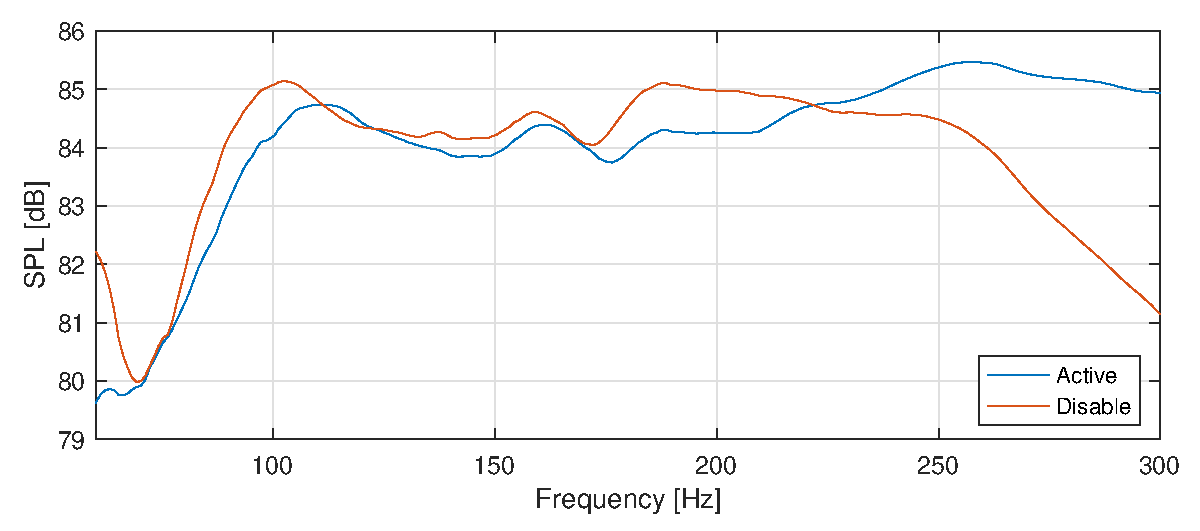
\includegraphics[width=1\textwidth]{beamforming_off_on.eps}
	\caption{The figure shows the \gls{spl} in front for the array with a distance of \SI{4.92}{\meter}, where the blue graph is with beamforming and the red graph is without beamforming}
		\label{fig:beamforming_off_on}
\end{figure}








because of the change the cost filter might have to be changed 


 \begin{figure}[H]
	\centering
	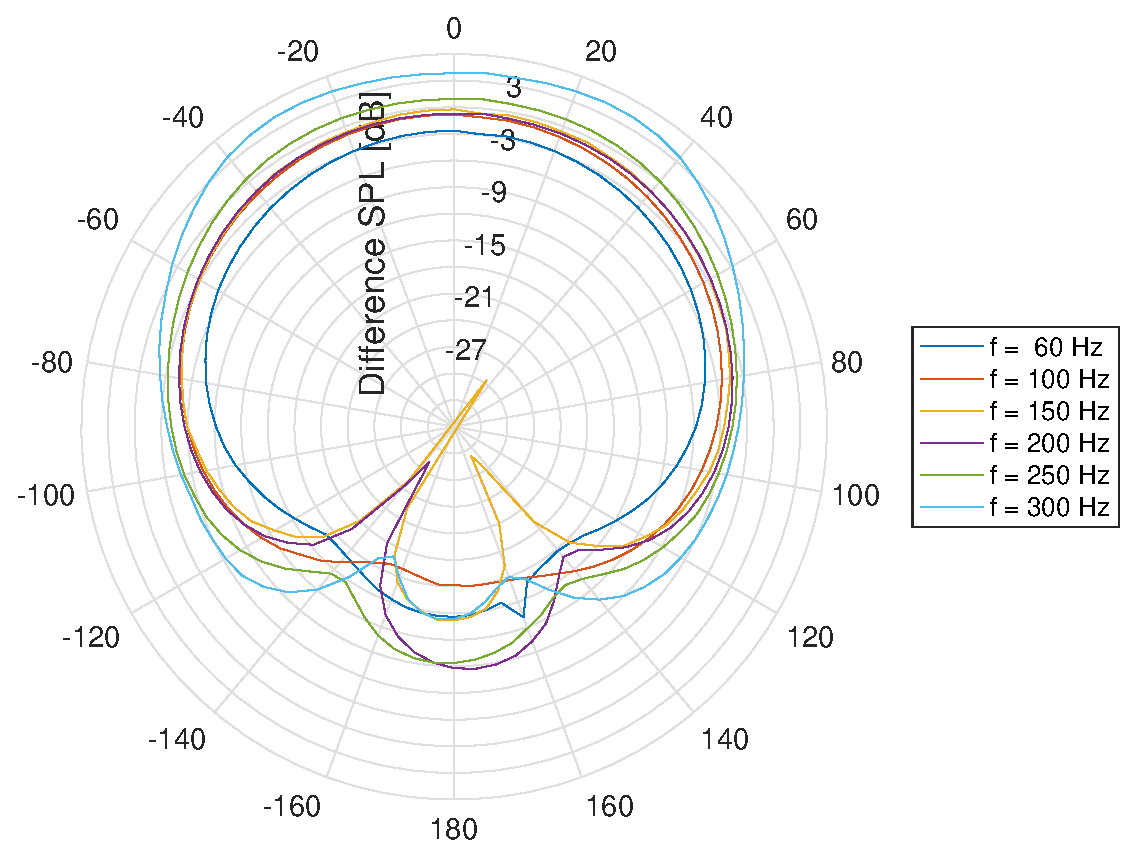
\includegraphics[width=0.8\textwidth]{polar_plot_dif_result.eps}
	\caption{The figure shows the \gls{spl} in front for the array with a distance of \SI{4.92}{\meter}, where the blue graph is with beamforming and the red graph is without beamforming}
		\label{fig:polar_plot_dif_result}
\end{figure}


instead of using the case in autoref{} it was desided to use a direct comparing 

other stand

direct comparing.